\subsection{Formación de imágenes}

Las \textbf{imágenes} se forman ya sea por \hl{reflexión} o \hl{refracción}, y es posible diseñar espejos y lentes que formen imágenes reales o virtuales.

\subsubsection{Introducción a los espejos}

\begin{wrapfigure}{r}{0.3\textwidth}
  \centering
  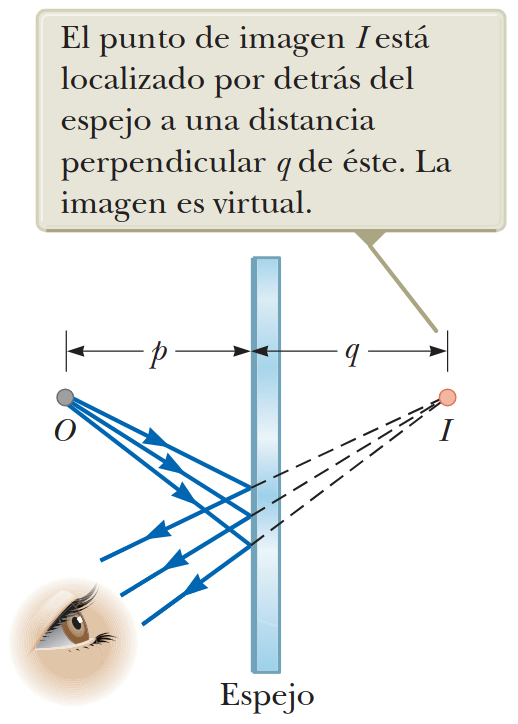
\includegraphics[width=\linewidth]{mirror.png}
  \caption{Imagen formada por reflexión en un espejo plano.}
  \label{fig:mirror}
\end{wrapfigure}
Los espejos forman imágenes a partir de la \textbf{reflexión} de la luz. Para entender cómo se forman las imágenes en un espejo, es importante entender los conceptos de reflexión y ángulos de incidencia y reflexión del haz de luz (ver sección \ref{sec:reflection}).

Cuando un rayo de luz incide sobre la superficie reflectante de un espejo, se refleja y puede llegar al ojo del observador. La \textbf{imagen} se forma en el punto donde los rayos reflejados (o sus prolongaciones) se interceptan.

\paragraph{Espejo plano}

Empecemos con la consideración del espejo más simple posible, el espejo plano. Imagine una fuente puntual de luz colocada en \(O\) en la figura \ref{fig:mirror}, a una distancia \(p\) de la superficie del espejo plano. La distancia \(p\) se llama \textbf{distancia objeto}. Los rayos luminosos \textit{divergentes}\footnote{Los rayos luminosos divergentes son aquellos que se alejan entre sí.} son reflejados por el espejo. Después de reflejarse, siguen un proceso de divergencia. Las líneas discontinuas de la figura \ref{fig:mirror} son extensiones de los rayos divergentes hacia atrás, hasta un punto \(I\), que se llama \textbf{imagen} del objeto \(O\). A la distancia \(q\) se la llama \textbf{distancia imagen}. 

Las imágenes están localizadas ya sea en un punto a partir del cual los rayos luminosos \textit{realmente} divergen, o en un punto a partir del cual los rayos luminosos \textit{aparentemente} divergen.

\begin{tcolorbox}[myconclusion]
    Independientemente del sistema de estudio, siempre se localizará las imágenes extendiendo hacia atrás los rayos divergentes, hasta el punto en que hacen intersección.
\end{tcolorbox}


\subsubsection{Imágenes reales y virtuales}

Las imágenes pueden clasificarse según varias características, una de ellas es si son \textit{reales} o \textit{virtuales}. Una imagen real es la que se forma cuando los rayos luminosos pasan por el punto de la imagen. Por otro lado, una imagen virtual es la que se forma cuando los rayos luminosos no pasan por el punto de la imagen, sino que parecen divergir desde el punto de la imagen. La imagen formada por el espejo de la figura \ref{fig:mirror} es virtual y está detrás del espejo.

La imagen vista de un objeto en un espejo plano \textit{siempre} es virtual.